\chapter{Material and method}
\label{chap:m&m}

\section{Material}

\subsection{Laboratory instruments}
BD Accuri C6 Plus benchtop flow cytometer (BD Nordics (prev. Puls Norway), Norway). Filters and lasers.
CytoSub submersible flow cytometer (CytoBuoy, Netherlands)
Coulter Counter Multisizer4 (Beckman Coulter, US) eqipped with a 100 \micro m aperature (size-range 2-60 \micro m)
Nikon Eclipse Ni-U Upright Microscope equipped with a CMOS camera (MC170HD, Leica Microsystems, Germany), [Filters: Nikon Brightline GFP-4050B filter-cube (channel 6), Objectives: Plan Fluor 40x/0.75 water immersion objective, Plan Fluor 100x/1.30 Oil immersion objective]
Leitz Labrolux 12 binocular microscope (Leica Mikroskopi AS, Norway) [EF 40/0.65 objective]
Eppendorf Centrifuge 5804 R (Eppendorf, Norway), [rotor: A-4-44, rotor radius: 15.5 cm], high-speed refrigerated benchtop centrifuge
Jouan KR22i floor centrifuge (Thermo Fischer Scientific, US), high-speed high capacity refrigerated floor centrifuge 8 [rotor: AK 100-21] angle?
Bürker Counting Chamber (Hirschmann Laborgeräte, Germany) with 0.1 mm depth of chamber
Eirik Lund sitt kamera, lense og imaging software: 
Sony ILCE A6400 with E-mount, lense: Tamron 17-70mm F/2.8 
Adobe\textsuperscript{\textregistered} Lightroom Classic 12.0 

\begin{table}[H]
	\centering
	%\caption{Chemicals used in the master thesis, listed alphabetically according to chemical name, including the chemical's CAS nr., purity/grade, supplier and state.}
	\label{tb:instruments}
	\resizebox{\linewidth}{!}{
	\begin{tabular}{lll}
	\textbf{Instrument} & \textbf{Commercial name} & \textbf{Producer} \\
		\midrule
   Benchtop Flow Cytometer               & BD Accuri$^{TM}$ C6 Plus & BD Biosciences \\
   Submersible Flow Cytometer            & Cytosub                  & CytoBuoy \\
   Coulter Counter                       & Multisizer 4             & Beckman Coulter \\
   Upright microscope                    & Eclipse Ni-U             & Nikon \\
   Transmitted/incident light microscope & Labrolux 12              & Leitz \\
   CMOS camera                           & MC170HD                  & Leica Microsystems \\
   Benchtop centrifuge                   & Centrifuge 5804 R        & Eppendorf\\
   Floor centrifuge                      & KR22i                    & Jouan \\
   Counting chamber                      & Bürker                   & Hirschmann \\
   		\bottomrule
	\end{tabular}
	}
\end{table}


\subsection{Chemicals}
\begin{table}[H]
	\centering
	%\caption{Chemicals used in the master thesis, listed alphabetically according to chemical name, including the chemical's CAS nr., purity/grade, supplier and state.}
	\label{tb:chemical-list}
	\resizebox{\linewidth}{!}{
	\begin{tabular}{lllll}
	\textbf{Chemicals (abbrv.)} & \textbf{CAS-No.} & \textbf{Purity/grade} & \textbf{Supplier} & \textbf{state} \\
		\midrule
    Calcium chloride dihydrate      & 10035-04-8 & $\geq$ 99.0 \% & Sigma Aldrich & s \\
    Dimethyl sulfoxide              & 67-68-5    & $\geq$ 99.5 \% & Sigma Aldrich & l \\
    D-(+)-Glucose                   & 50-99-7    & $\geq$ 99.5    & Sigma Aldrich & s \\
    EDTA anhydrous                  & 60-00-4    & $\geq$ 99 \%   & Sigma Aldrich & s \\
    \ce{Na2EDTA}$\cdot$\ce{2H2O}    & 6381-92-6  & 98.5-101.5 \%  & Sigma Aldrich & s \\
    Ethanol                         & 64-17-5    & 96 \% vol      & VWR           & l \\
    Formaldehyde                    & 50-00-0    & 37\% wt        & Sigma Aldrich & l \\
    HEPES                           & 7365-45-9  & $\geq$ 99.5 \% & Sigma Aldrich & s \\
    Magnesium sulfate heptahydrate  & 10034-99-8 & $\geq$ 99.5 \% & Sigma Aldrich & s \\
    Methanol                        & 67-56-1    & $\geq$ 99.9 \% & Sigma Aldrich & l \\
    Potassium chloride              & 7447-40-7  & $\geq$ 99.9 \% & Sigma Aldrich & s \\
    Sodium chloride                 & 7647-14-5  & $\geq$ 99.5 \% & Merck         & s \\
    TRIS(hydroxymethyl)aminomethane & 77-86-1    & ACS reagent    & Merck         & s \\
    TRIS HCl                        & 1185-53-1  & $\geq$ 99.0 \% & Sigma Aldrich & s \\
		\bottomrule
	\end{tabular}
	}
\end{table}


\subsection{Reagents for Flow Cytometry}
\begin{table}[H]
	\centering
	%\caption{Reagents and kits used in the master thesis, listed alphabetically according to product name, including manufacturer, supplier and supplier's catalogue number.}
	\label{tb:reagent-list}
	\resizebox{\linewidth}{!}{
	\begin{tabular}{lllll}
	\textbf{Product name (abbrv.)} & \textbf{Manufacturer} & \textbf{Supplier} & \textbf{Catalogue} & \textbf{Dilution} \\
		\midrule
    TO-PRO-3 &  InVitrogen$^{TM}$  & Thermo Fisher	& T3605 & 1:20 \\
    Ethidium Homodimer-1 &  InVitrogen$^{TM}$ & Thermo Fisher &  E1169 & 4 \micro L/sample \\
    Apotracker$^{TM}$ Green & BioLegend & Fisher Scientific & 50-207-9934 & NA \\
    Calcein-AM & Invitrogen$^{TM}$ & Thermo Fisher & C1430 & 1:80 \\ 
    CS\&T RUO beads & BD Biosciences & BD Biosciences & 661414 &  4 drops/mL \\
    8-peak validation beads & Spherotech & BD Biosciences & 653144 & 4 drops/mL \\
    6-peak validation beads & Spherotech & BD Biosciences & 653145 & 4 drops/mL \\
		\bottomrule
	\end{tabular}
	}
\end{table}


\subsection{Microscopy kits and reagents}
\begin{table}[H]
	\centering
	%\caption{Reagents and kits used in the master thesis, listed alphabetically according to product name, including manufacturer, supplier and supplier's catalogue number.}
	\label{tb:Microscopy-list}
	\resizebox{\linewidth}{!}{
	\begin{tabular}{llll}
	\textbf{Product name (abbrv.)} & \textbf{Producer} & \textbf{Supplier} & \textbf{Catalogue} \\
		\midrule
    Giemsa's azur eosin methylene blue solution & Merck & Sigma Aldrich & 1.09204.0500 \\
    Hemacolor\textsuperscript{\textregistered} & Sigma Aldrich & Sigma Aldrich & 1.11661 \\
    Eukitt\textsuperscript{\textregistered} Quick-hardening mounting medium & Orsatec GmbH & Sigma Aldrich & 03989 \\
    Type N Immersion Oil for Microscopy & Nikon & ? & MXA20234 \\
    Methanol & Merck & Sigma Aldrich & 1.06009.2511 \\
    4\% formaldehyde in MAS &&& \\
    Percoll$^{TM}$ & Cytiva Sweden AB & Sigma Aldrich & GE17-0891-02 \\
    Centrifuge tubes, Oak Ridge, 50 mL & Nalgene\textsuperscript{\textregistered} & VWR & 525-0046 \\
		\bottomrule
	\end{tabular}
	}
\end{table}






\subsection{Buffers and solutions}
\begin{table}[H]
	\centering
	\label{tb:buffers}
	\resizebox{\linewidth}{!}{
	\begin{tabular}{ll}
	\textbf{Buffer} & \textbf{Composition} \\
		\midrule
    MAS                   &  375.6 mM \ce{NaCl}, 28.97 mM Citric Acid$\cdot$3Na$\cdot$2\ce{H2O}, 113.8 mM D-Glucose, \\ 
                          & 2.617 mM Citric Acid$\cdot$\ce{H2O}, 11.5 mM \ce{Na2EDTA}$\cdot$\ce{2H2O}, pH=7.0 \\
    Anticoagulant buffer  & 55.5 mM D-glucose, 171.1 mM NaCl, 13.43 mM \ce{Na2EDTA}$\cdot$\ce{2H2O}, \\
                          & 0.05 M TRIS/HCl, pH=7.6 \\ 
    PBS                                  & 136.9 mM \ce{NaCl}, 2.7 mM \ce{KCl}, 10.1 mM \ce{Na2HPO4}, 1.8 mM \ce{KH2PO4} \\
    Sorensen Buffer       & 66.67 mM \ce{KH2PO4}, 66.67 mM \ce{Na2HPO4}$\cdot$\ce{2H2O}, pH=6.8 \\
    Leibovitz-15          &                                              \\
    HBSS                  &                                              \\
    Hemolymph solution    &  470 mM \ce{NaCl}, 10 mM \ce{KCl}, 10 mM \ce{CaCl2}, 10 mM HEPES \\
                          & 47.7 mM \ce{MgSO4}, pH=7.41 \\
		\bottomrule
	\end{tabular}
	}
\end{table}

\section{Method}
\subsection{Experimental setup/}
\emph{Mytilus edulis} (mean+-SD shell length cm and age?) were obtained from Snadder og Snaskum AS (Indre Fosen, Norway), transportation, that the supplier were asked not to shrub the shells, animal housing prior to experiment (erated, flow through volume, temperature, water type/source, time period, feeding, did they attach with byssus?), decribe depuration period

\subsection{Hemolymph sampling technique}
To minimize the possibility of contaminating hemolymph samples during extraction, a simple and time-effective sampling technique modified from the nonlethal technique of Gustafson et al., 2005 was developed. A "blind" method of withdrawal through a notch in the posterior dorsal shell or through the exhalant syphon frequently resulted in considerable contamination with debris from the pallial fluid or the lungs (data not shown). Therefore, the hemolymph sampling technique employed was centered around achieving good visual contact with the posterior adductor muscle and the position of the needle within the muscle during hemolymph withdrawal, and was mainly constricted by the requirement of an intact digestive gland.

The digestive gland is located dorsally (towards the hinge), slightly off-center towards the anterior end (Eggermont, 2020). In order to access and see the posterior adductor muscle while staying clear of the digestive gland, the valves were prised apart ventrally by gently forcing a tissue forceps between the valves midway of the mussel's length, or slightly posterior of the byssal mass (Fig. \ref{fig:Hemolymph_sampling_illustration}a). When the pallial cavity opened, pallial fluid (seawater) was drained away from the posterior adductor muscle by positioning the mussel's umbo on a paper tissue for 15-30 seconds. Since the posterior adductor muscle is oblong in the anteroposterior direction, penetrating the muscle from the posterior end pointing straight anteriorly gave the operator better margins to avoid piercing the muscle. To create a free path to the muscle from the posterior direction, the connecting mantle immediately surrounding the exhalant syphon where cut with a scalpel (Fig. \ref{fig:Hemolymph_sampling_illustration}b and d), holding the blunt spine of the scalpel blade facing the posterior adductor muscle.  Thus, when illuminating the pallial cavity from above with the ventral aspect facing upwards, the operator was able to supervise the position of the needle in the muscle sinus through the slightly transparent muscle fibers, as seen in Fig. \ref{fig:Hemolymph_sampling_illustration}c. The mussels were placed in the palm of the operator's non-dominant arm, 3$^{rd}$-5$^{th}$ digits firmly gripping the mussel, first and second digits holding the syringe steady in the anteroposterior direction, while the dominant arm were used to withdraw the syringe plunger.

\begin{figure}
    \centering
    \begin{subfigure}[b]{.45\textwidth}
        \centering
        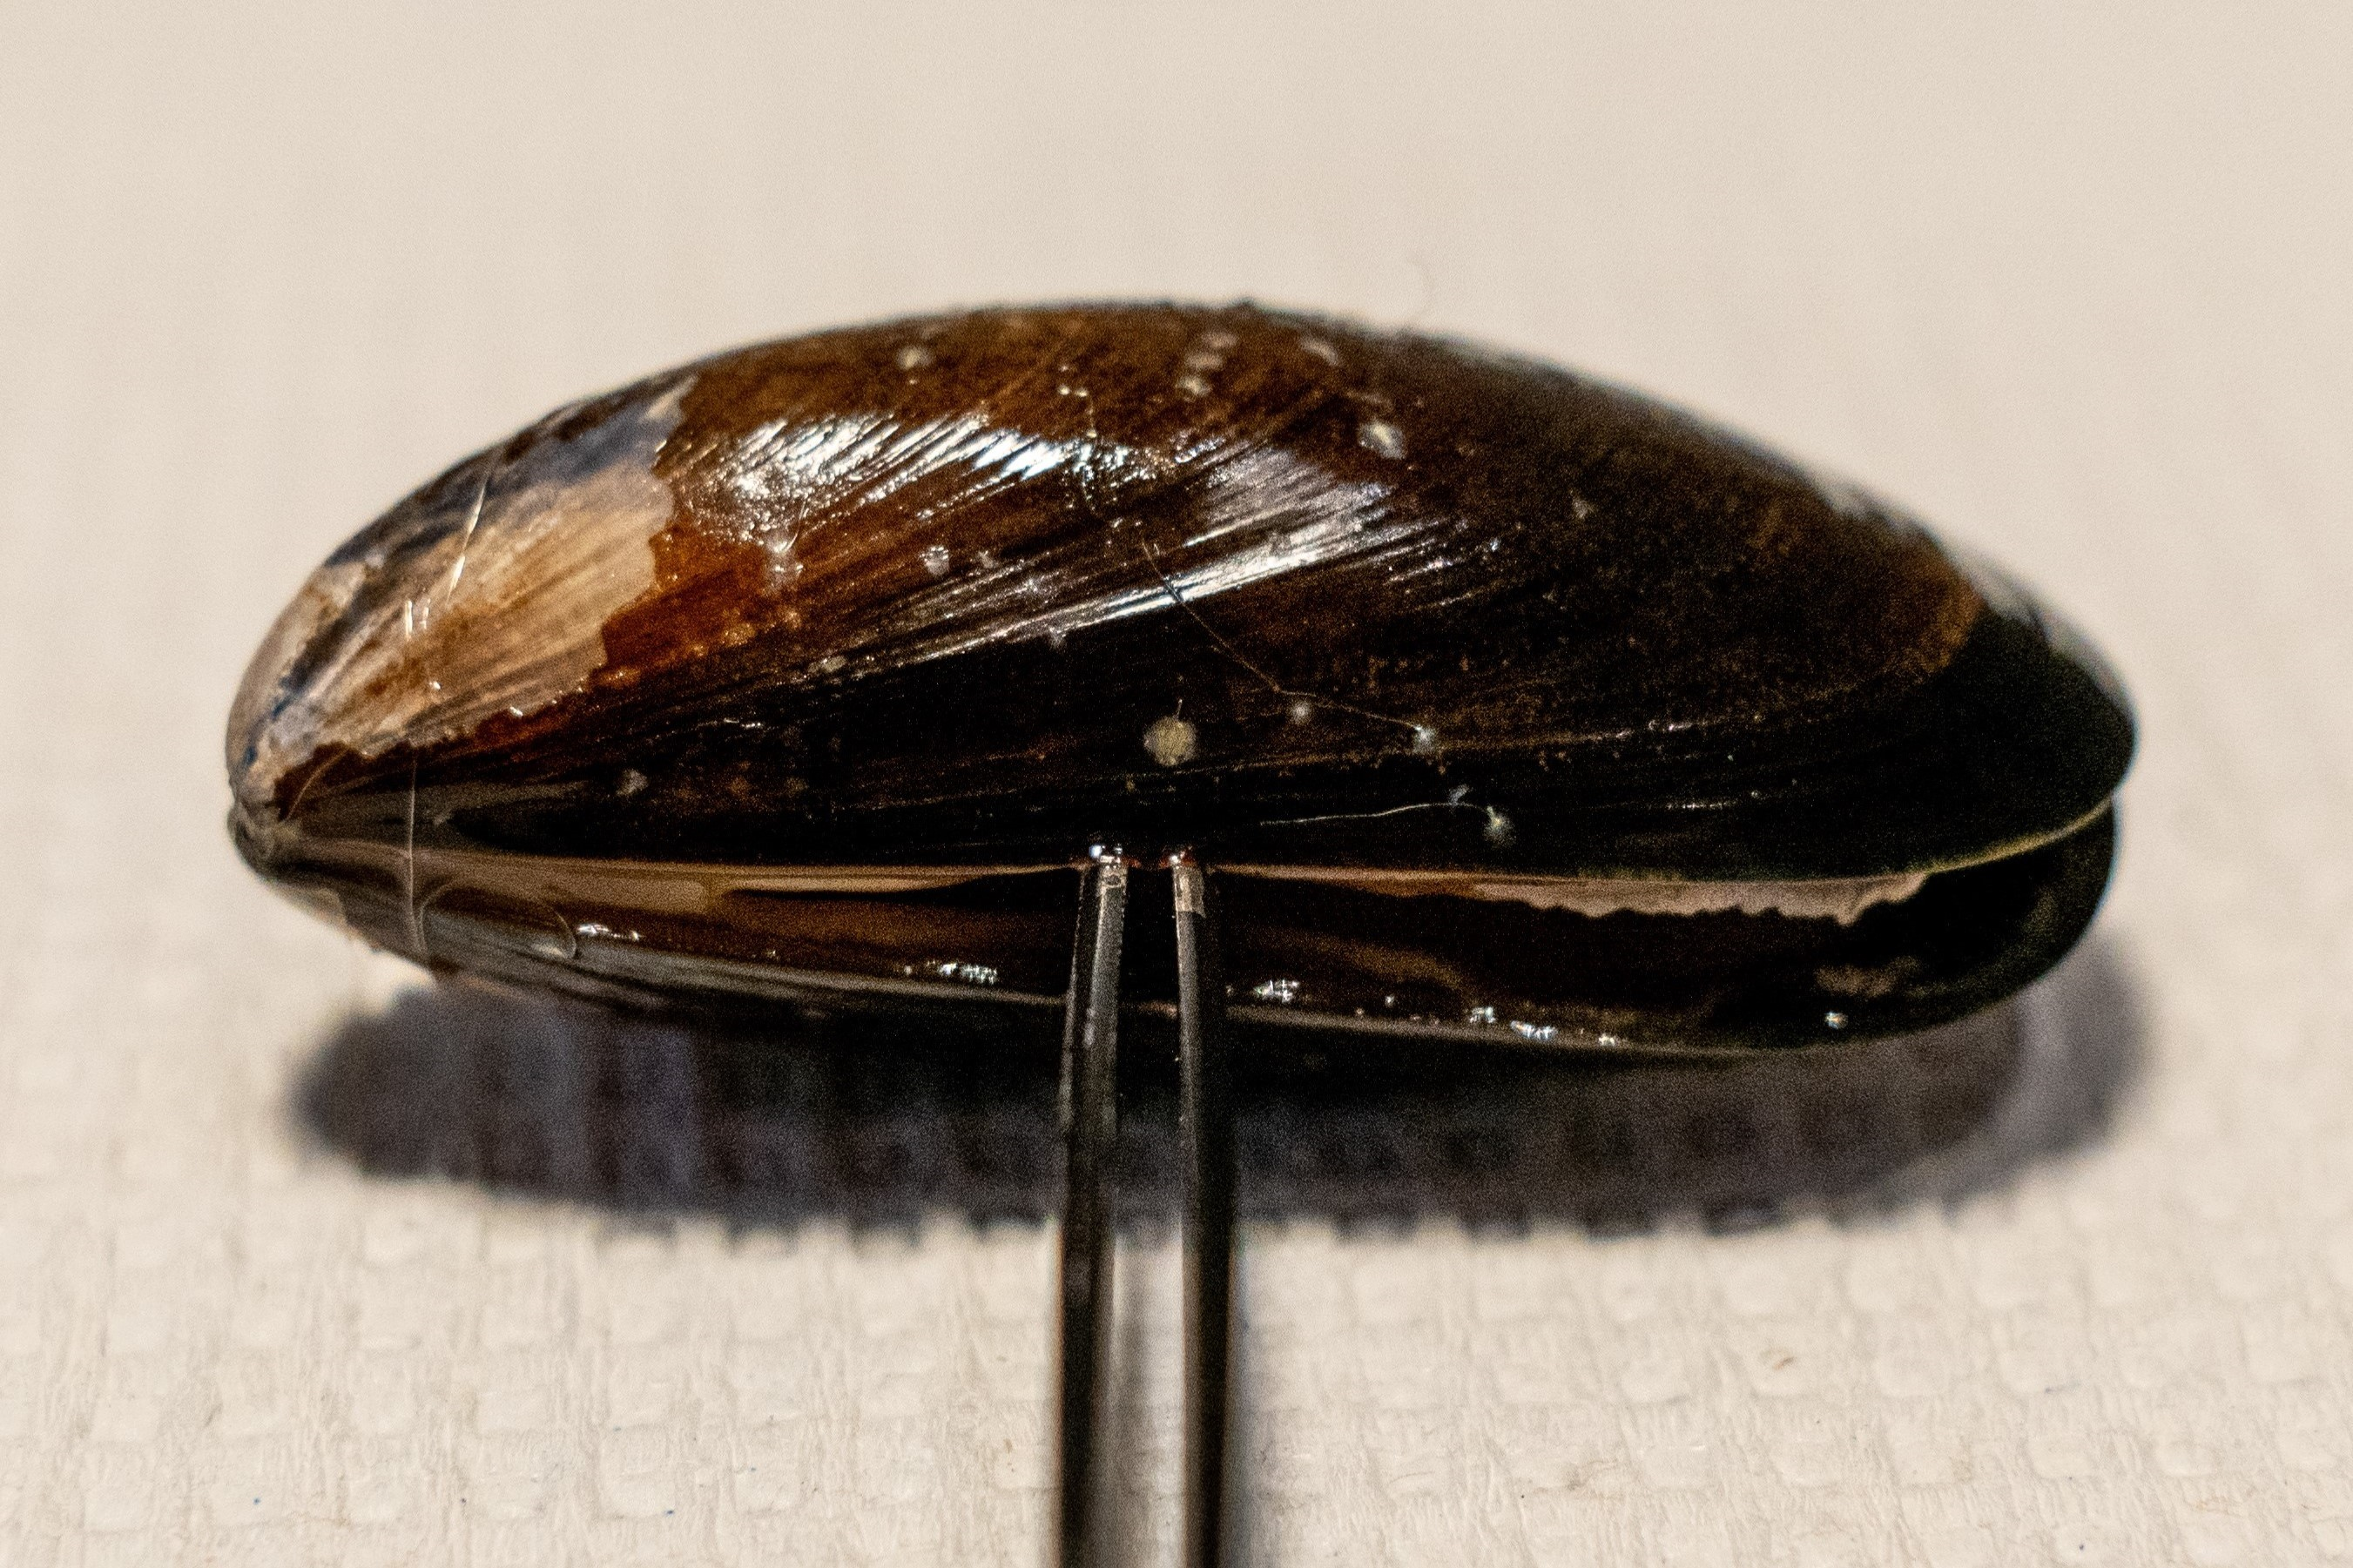
\includegraphics[width=\textwidth]{figures/Sampling technique/forceps square color.jpg}
        \caption{Placement of forceps between valves on the ventral side of the mussel.}
        \label{sfig:a}
    \end{subfigure}
    \hfill
    \begin{subfigure}[b]{.45\textwidth}
        \centering
        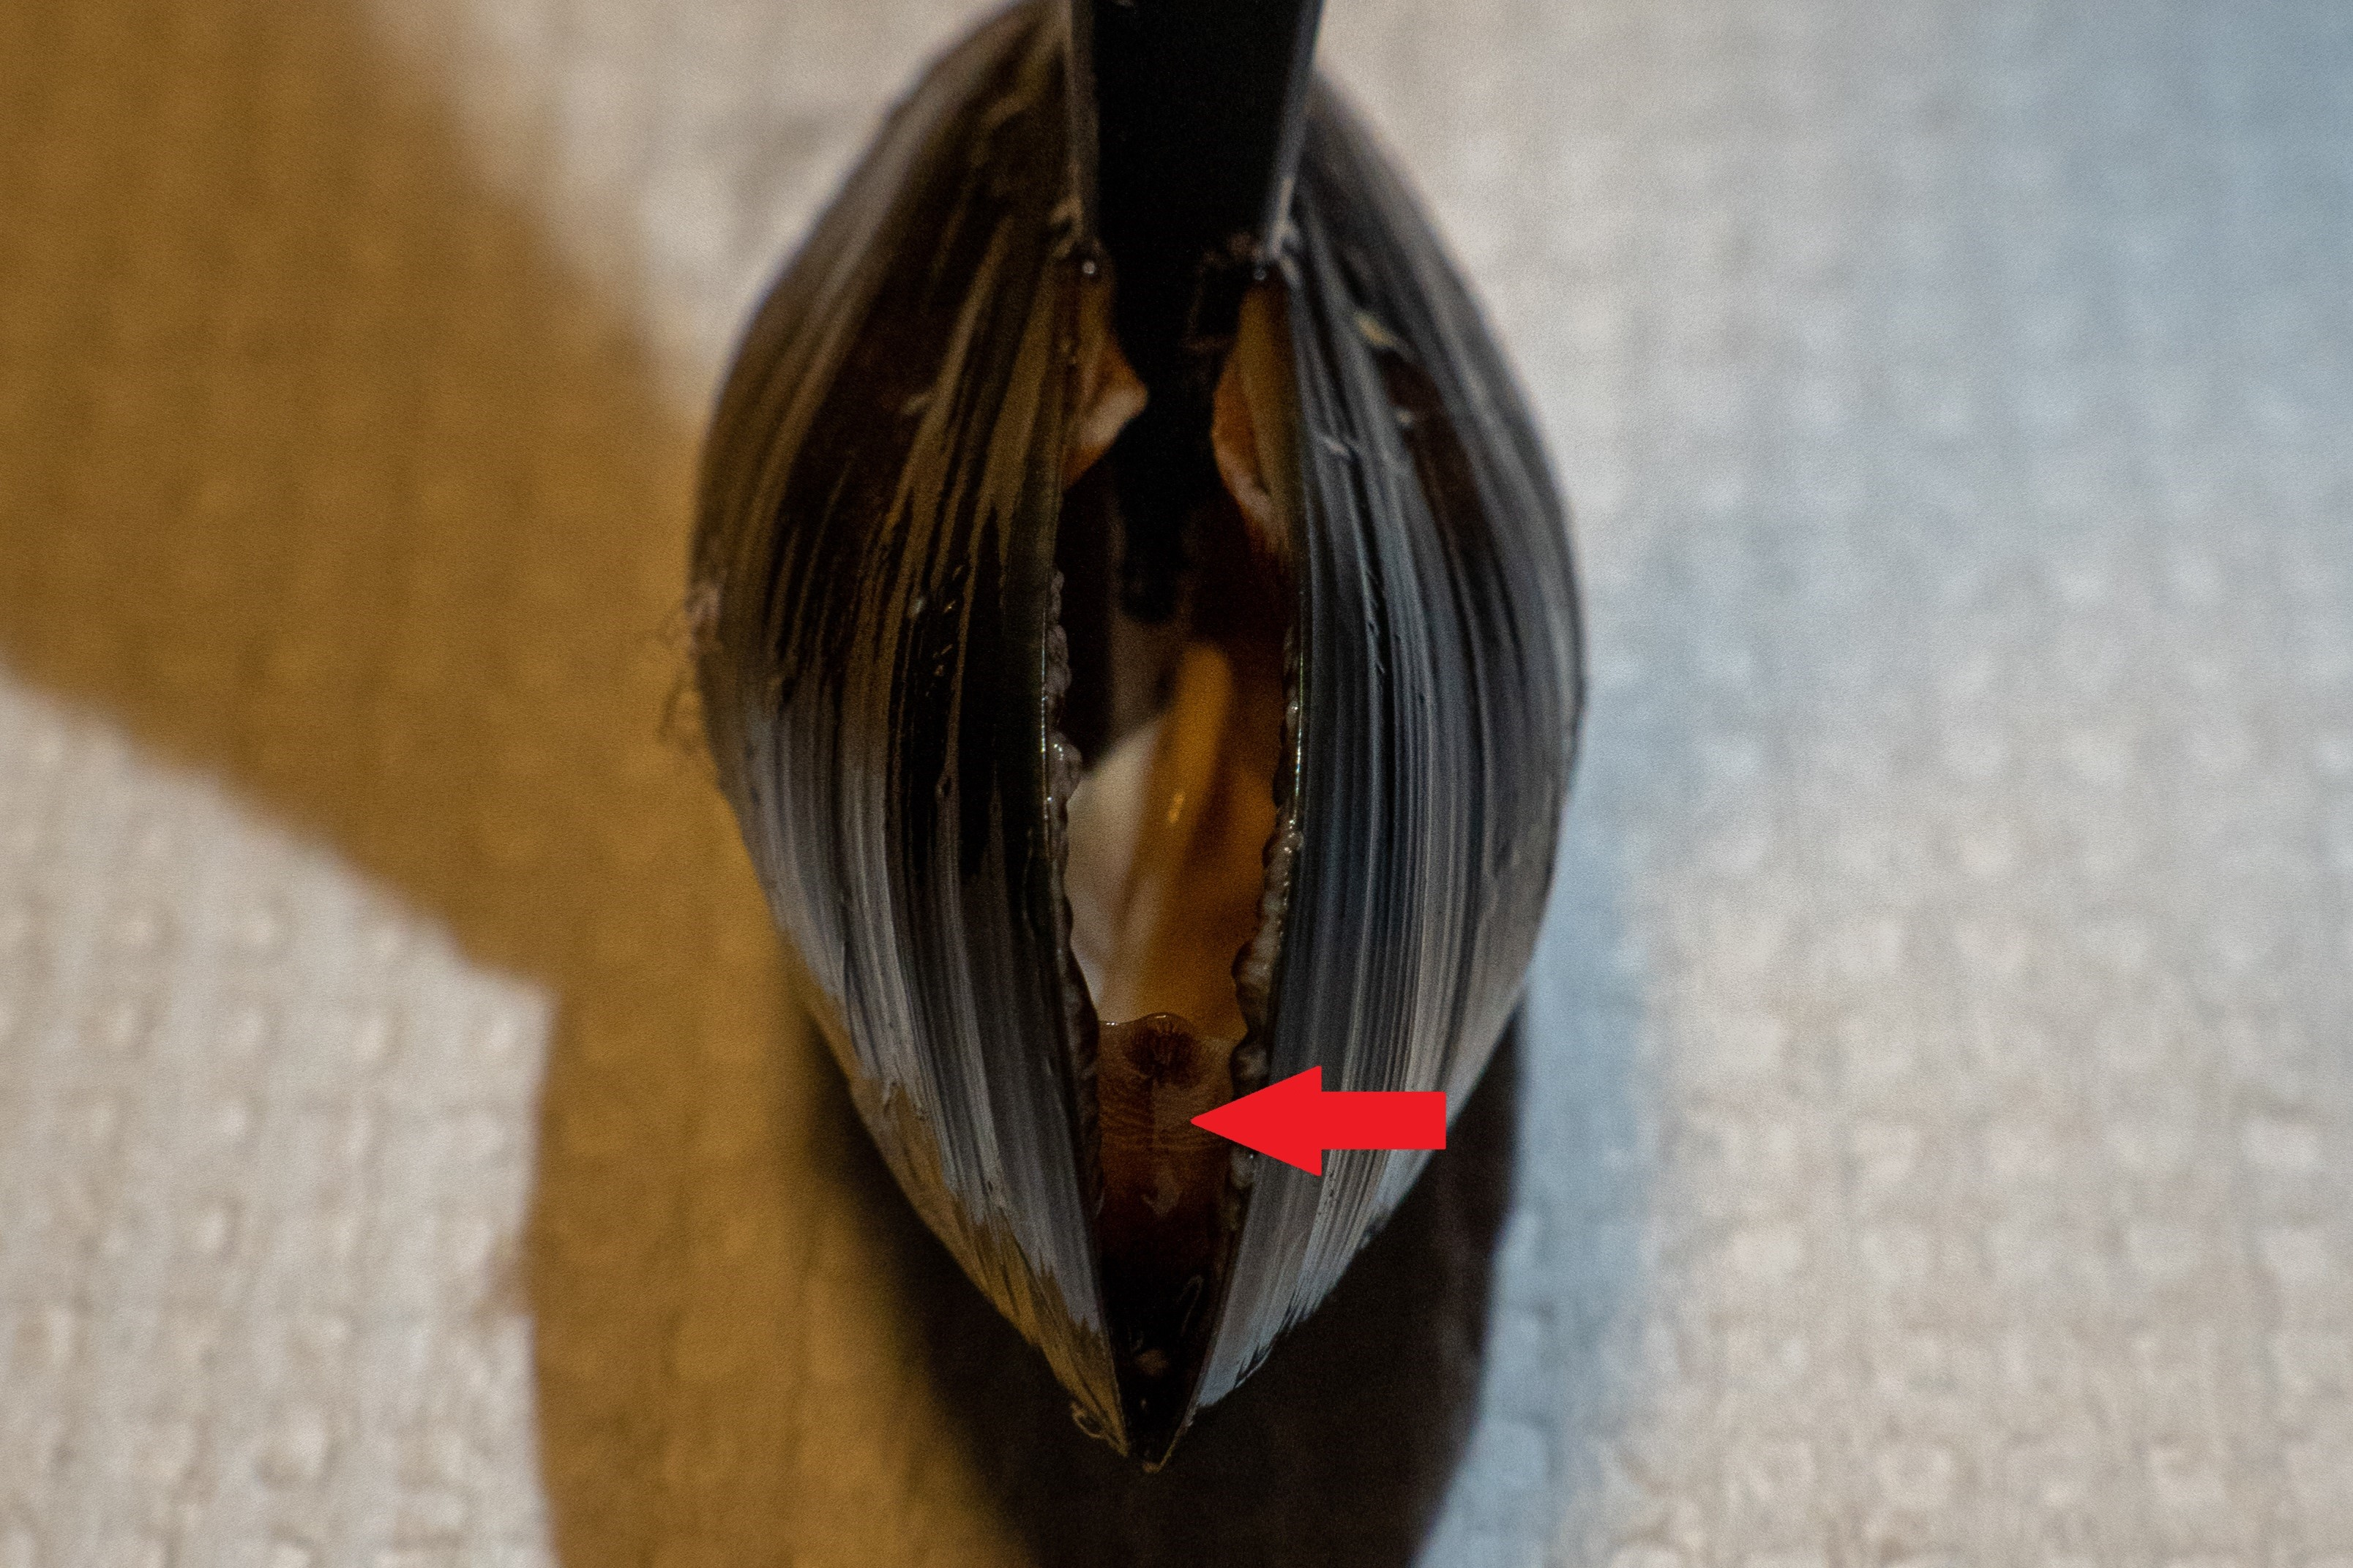
\includegraphics[width=\textwidth]{figures/Sampling technique/uncut color 3495.jpg}
        \caption{Posterior aspect of mussel with the connecting mantle (red arrow) intact.}
        \label{sfig:b}
    \end{subfigure}
    \newline
    \begin{subfigure}[b]{.45\textwidth}
        \centering
        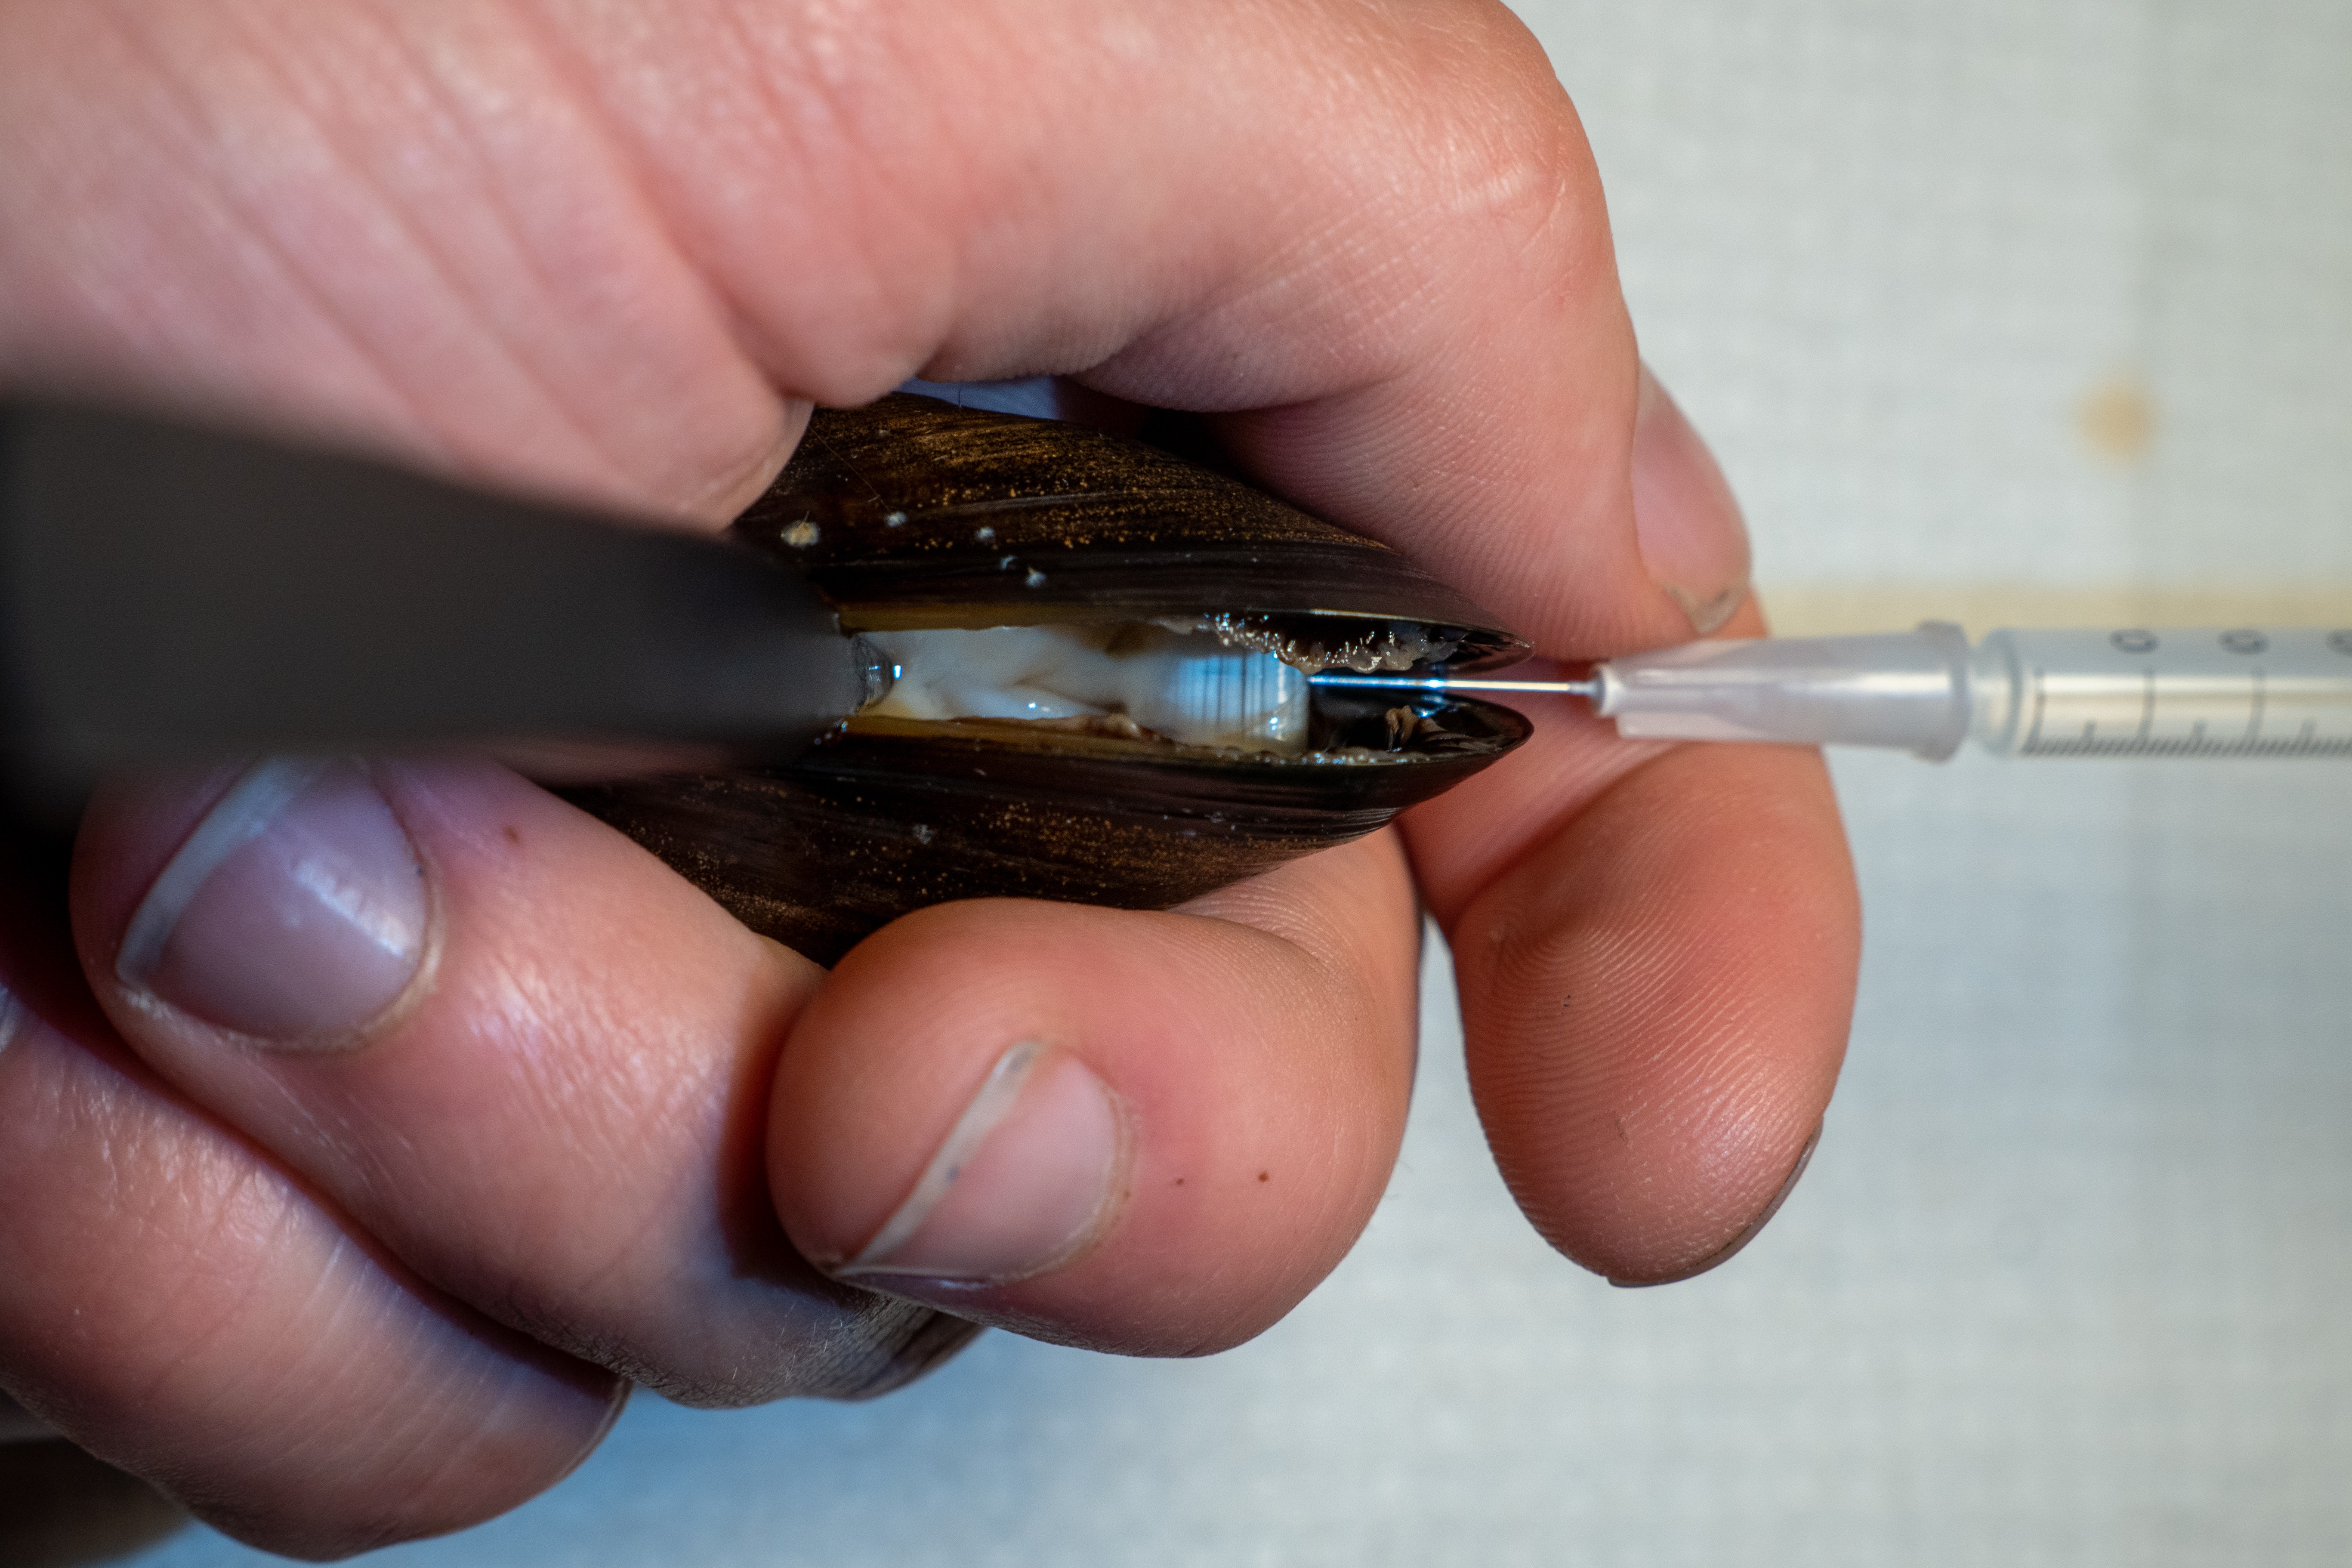
\includegraphics[width=\textwidth]{figures/Sampling technique/hands colors centered.jpg}
        \caption{The mussel grip and needle alignment employed, seen from the operators perspective. }
        \label{sfig:c}
    \end{subfigure}
    \hfill
    \begin{subfigure}[b]{.45\textwidth}
        \centering
        \includegraphics[width=\textwidth]{figures/Sampling technique/possible match.jpg}
        \caption{Mussel with visible posterior adductor muscle (red arrow) where the mantel was cut.}
        \label{sfig:d}
    \end{subfigure}
    \caption{An illustration of the method employed to extract hemolymph from M. edulis in order to avoid off-target withdrawal of fluid from the lungs or remaining pallial fluid. The pictures were taken using a Sony A6400 mirrorless digital camera with a Tamron 17-70mm F/2.8 lens, and edited with Adobe\textsuperscript{\textregistered} Lightroom Classic 12.0 image editing software.}
    \label{fig:Hemolymph_sampling_illustration}
\end{figure}

\subsection{Selection of hemocyte medium}
The hemocytes of \emph{M. edulis} have a tendency to form aggregates upon mechanical stress, e.g. when the hemolymph is withdrawn through a thin syringe needle. Since accurate flow cytometric quantifications rely on single-cell measurements, there was a need to minimize hemocyte aggregation occurring from hemolymph withdrawal during staining procedures, until the samples could by analyzed on the flow cytometer. In the literature, several authors have dealt with this problem by aspirating hemolymph samples directly into slightly acidic EDTA-containing solutions buffered by citric acid (\cite{Söderhall1983, Bachere1988, LeFoll2010}). Since hemocyte aggregation is a Ca$^{2+}$-dependent process (\cite{Rolton2020}), withdrawal of hemolymph into an EDTA-containing buffer effectively slows the rate of hemocyte aggregation, although it does not inhibit aggregation completely. [Include tests to investigate if EDTA alters hemocyte viability within 15 minutes or if it effects cytograms]. Another frequently reported method is to withdraw the hemolymph into cold filtered seawater (FSW), while keeping the samples on ice until analysis.

In search for the most effective method for this work, hemolymph samples were withdrawn into syringes pre-filled with a number of different "anticoagulant" or "antiaggregative" buffers (1:1) reported in the literature. After preliminary testing, the most promising buffers encountered where the Modified Alsever's Solution (MAS, pH=6.2) with ethylenediaminetetraacetic acid (EDTA) and citric acid reported by \cite{LeFoll2010}, and the similar Anticoagulant Buffer (ACB, pH=7.6) with EDTA reported by \cite{Pipe1997}. Since these three factors (EDTA and/or low pH or keeping samples on ice) might introduce inconveniences related to staining procedures, an experiment was devised in order to test their effect on hemocyte aggregation under the conditions intended for our FCM analysis, such that a cost-effect assessment could be performed. The experiment was seeded from the observation that FCM singlet hemocyte counts tended to decrease over time from hemolymph withdrawal, and were based on the assumption that the decrease was caused by aggregation alone. Thus, the proportion of aggregated hemocytes in a sample at a given time could be retraced from the initial hemocyte count when performing several counts of the same sample over time. 

250 \micro L hemolymph was withdrawn from 23 individual mussels into 250 \micro L Hemolymph saline (HLS, n=8) on ice, MAS (n=7) or ACB (n=8), and the number of singlet hemocyte events were determined by acquiring 20 \micro L sample on the FCM immediately thereafter. Each sample was run with identical acquisition and FCM fluidics settings (see table \ref{tb:FCM_settings}), with a doublet exclusion gate and FSC-A vs. SSC-A hemocyte gate held constant. To account for any extra aggregation occurring from gentle mixing with any flow cytometry reagents, the samples were added 6 \micro L 1 \micro M TO-PRO-3 iodide and incubated for 15 minutes before the second measurement. Three more singlet hemocyte counts where recorded of each sample at 30, 45 and 60 minutes post-withdrawal, to discern the buffers' ability to prevent aggregation during longer incubation periods.

To test the experimental assumption of aggregation as the sole mechanism behind decreases in hemocyte counts, four hemocyte samples were moderately shaken to suspend any sedimented hemocytes before sample acquisition. This further increased the rate of aggregation (data not shown), which ruled out sedimentation as an important mechanism. Being the only other mechanism conceivably involved, the assumption was regarded as valid under the current experimental conditions.

The proportion of aggregated hemocytes where calculated according to equation \ref{eq: proportion_agg}.

\begin{equation}
    \label{eq: proportion_agg}
    \hat{p} = \dfrac{N_{t0} - N_{tx}}{(N_{t0} - N_{tx}) + N_{tx}} = \dfrac{N_{t0} - N_{tx}}{N_{t0}}
\end{equation}

\begin{equation}
    \label{eq:agg_free_matrix}
    y = 
    \begin{pmatrix}
      N_{t0_{1}} - N_{tx_{1}} &  N_{t0_{1}} \\
      N_{t0_{2}} - N_{tx_{2}} &  N_{t0_{2}} \\
      N_{t0_{3}} - N_{tx_{3}} &  N_{t0_{3}} \\
      \vdots                   & \vdots       \\
      N_{t0_{n}} - N_{tx_{n}} &  N_{t0_{n}} \\
    \end{pmatrix}
\end{equation}
\
Where $\hat{p}$ is the proportion of aggregated hemocytes, N$_{to}$ is the initial number of singlet hemocytes in the sample and N$_{tx}$ is the number of singlet hemocytes at time x after hemolymph withdrawal. The proportion of aggregated hemocytes were modelled as a function of log time, with buffer as a categorical explanatory variable, using the base R glm() function with a "quasibinomial" error distribution and "logit" link function, as shown in Code listing 3.1. Instead of using the calculated proportions ($\hat{p}$), the response variable was formatted as a two-column matrix of aggregated and singlet hemocyte counts (see equation \ref{eq:agg_free_matrix}), such that logistic regression was possible. The logistic GLM model coded the categorical explanatory variable's factor levels into dummy variables (see equation \ref{eq:dummy_variables}), and used the MAS buffer as reference level. The resultant logistic model can be written out as in equation \ref{eq:logit} on the original scale, where $\alpha + \beta_{1}x_{i}$ is the linear predictor of the reference level, $\alpha_{2}$ and $\alpha_{3}$ are the difference in y-intercept for the HLS and ACB buffers, while $\beta_{2}$ and $\beta_{3}$ are the differences in slopes for the same buffers, respectively. The data is presented in figure \ref{fig:aggregation}, together with the three buffers' "sub-models".

\begin{lstlisting}[language=R, caption = {The R source code run to fit the logistic proportion aggregation model.}]
model = glm(y ~ log(t) + Buffer + log(t):Buffer,
family = quasibinomial(link = "logit")
\end{lstlisting}

\begin{equation}
    \label{eq:dummy_variables}
D_{2} =\begin{cases}
      1, & \text{HLS}\\
      0, & \text{not HLS},
    \end{cases}
    \quad
D_{3} =\begin{cases}
      1, & \text{ACB}\\
      0, & \text{not ACB}
    \end{cases}
\end{equation}

\begin{equation}
\label{eq:logit}
\hat{p}_{i} = \dfrac{1}{1 + e^{-(\alpha \: + \: \beta_{1} x_{i} \: + \: \alpha_{2} D_{2} \: + \: \alpha_{3} D_{3} \: + \: \beta_{2} D_{2} \: + \: \beta_{3} D_{3} \: + \: \epsilon_{i})}}
\end{equation}

\begin{figure}[!ht]
    \centering
    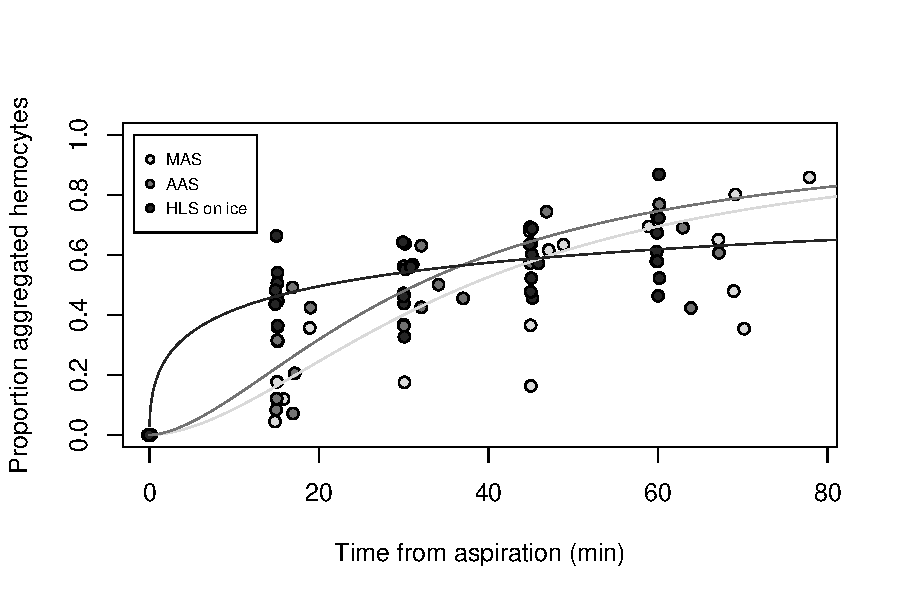
\includegraphics[width=1.0\textwidth]{figures/greys368.pdf}
    \caption{The proportion of aggregated \emph{M. edulis} hemocytes in hemolymph samples aspirated into 250 \micro L MAS (n=7), ACB (n=8) and HLS (n=8) buffers (1:1), plotted against time (min) after withdrawal from the posterior adductor muscle. The lines depict the proportion of aggregated hemocytes vs. time using the three different buffers, as predicted by the fitted logistic regression model.}
    \label{fig:aggregation}
\end{figure}

Interpreting the logistic sub-models, it evident that MAS and ACB effectively slowed the rate of aggregation during the first 30 minutes post-withdrawal. When MAS was used as a hemocyte medium, the predicted mean proportion of aggregated hemocytes after 20 minutes was 0.25, CI = (0.20, 0.30). This is not significantly different from the mean proportion when ACB was used (0.31, CI=(0.27, 0.37)), but both buffers containing EDTA had significantly lower hemocyte aggregation after 20 minutes compared to HLS (0.50, CI=(0.38, 0.61)). Although the model is over-dispersed, these estimates provided some insight into the three factor's relative abilities to prevent hemocyte aggregation. From these results, it was decided to draw all hemolymph samples into MAS (1:1). Since complete inhibition of hemocyte aggregation is unachievable, samples were run on the flow cytometer directly after staining procedures. Hemocytes that aggregated in spite of these efforts were gated out of analysis using a FSC-A vs. FSC-H doublet exclusion gate (see Gating Strategy). 

\subsection{Hemolymph Withdrawal/Extraction/Collection of hemolymph}
Using the method described above...
Technicalities of the withdrawal (1 mL syringes with 27 gauge hypodermic needles).
Syringe filled with 0.5 mL anticoagulant solution (ALS or AA).
[Should check if EDTA changes the cytogram, because it would be nice to report that it doesn't affect them.] 
Volume withdrawn, time used when aspirating these volumes
Dilution correction to 1:1 hemolymph:MAS after withdrawal if volume > 0.5 mL hemolymph. 
Hemolymph was not pooled or centrifuged (crude hemolymph). Report pH and osmolarity of the MAS buffer, and say that it is similar to the osmolarity of hemolymph/seawater 990 mOsm (Hartl, 2010). The osmolarity of MAS and ACB were adjusted to approximately 990 mOsm by the addition of \ce{NaCl}, to reflect that of \emph{M. edulis} hemolymph (Hartl, 2010)

\subsection{Determination of hemocyte concentration and subpopulations}
"The total hemocyte concentration, morphometry and definition of sub-populations were determined using side scatter (SSC) and forward scatter (FSC) light. Side scatter light corresponds to the relative internal complexity or granularity of the cells and FSC corresponds to the relative cell size" \cite{Rolton2020}
What did I use it for?

Scoring a defined subpopulation of hemocytes for nuclear anomalies by light microscopy is a time-consuming and labor-intensive process... Bridge to semi-automation: inter-operator variability, subjectivity etc.

With the BD Accuri C6 Plus benchtop flow cytometer, a maximum of three distinct hemocyte subpopulations (clusters) could be distinguished from the hemolymph on Forwards scatter (FCS) vs. Side scatter (SSC) dotplots. (don't oversell the FCM ability to distinguish them... In most adult mussels however, the basophilic and eosinophilic granulocyte subpopulations are partly or substantially overlapping. Since the BD Accuri C6 Plus isn't equipped with adjustable laser gain settings, these subpopulations could not be further separated instrumentally, and any attempt to gate on these subpopulations based solely on light scattering properties would introduce a considerable uncertainty. Since eosinophilic granulocytes produce/have more autofluorescence than the basophilic, and display higher density of granules (granularity), a bivariate plot of green fluorescence (518-548 nm) on log scale vs. SSC could accurately separate these subpopulations in about 1/10 of individuals (n=46, HMS data, data not shown), however the mean absolute error were [continue here]

Concider including the experiment that was performed to validate the BD Accuri C6 Plus hemocyte counting technique with a technique using counting beads. Mention that a hemocytometer/counting chamber was used for the initial method development. It's a lot of data and work, which never looks bad. [Maybe not a separate subsection, but include under FCM or elsewere?]

\subsection{Flow Cytometry}
Flow Cytometer used and Flow Cytometry acquisition software
External software used for graphing and analysis of exported FCS files.
Replicate/triplicate measurements?
Number of events recorded for each mussel? ()
Briefly describe FCS and SSC.
Mention if data were collected in linear or logarithmic scale, 
FSC treshold (80.000 FSC-H)
Fluorescent compensation (matrix)
Describe gating strategy herein? Debris exclusion; doublet exclusion --> hemocytes. (Gating of basophils and eosinophils, the use of FMO controls with TO-PRO-3 and/or the apoptosis stain) to create gates.

Theory behind Annexin-V/Apo-15: Annexin V
has affinity for phosphatidylserine, which is externalized to the
outer layer of the plasma membrane in the earlier stages of
apoptosis. Annexin V also binds internal phosphatidylserine in
permeable membranes, i.e. dead cells. Thus, dead cells are Apo-15+ ToPro3+, while the early apoptotiv cells are only Apo15+.

\begin{table}[H]
	\centering
	\caption{The FCM acquisition and fluidics settings specified with the BD Accuri C6 Plus acquisition software during the flow cytometric experiments reported in this work.}
	\label{tb:FCM_settings}
	\resizebox{\linewidth}{!}{
	\begin{tabular}{lllll}
	\textbf{Experiment nr.} & \textbf{Event-triggering threshold} & \textbf{Acquisition stop-condition} & \textbf{Flow rate (\micro L/min)} & \textbf{Core size (\micro m)} \\
		\midrule
    Aggregation & 80.000 FCM & acquired volume, 20 \micro L & 30 & 10 \\
    Fill & in & when & the experiment is set & completely \\
		\bottomrule
	\end{tabular}
	}
\end{table}

\subsection{Assay Validation}
Both dead cell stain and apoptosis stain has to be validated. For TO-PRO-3 perform the same experiment with 70\% methanol-killed cells as you did for Calcein-AM + EthD-1, and use Calcein-AM to stain live cells.
How to do this for the Apo-stain?

\subsection{Detecting }

\subsection{Measurements and calculations}
(\cite{R-project})